\pagenumbering{arabic} \setcounter{page}{1}
\chapter{Introduction}
\label{chap:intro}
% 1. legged locomotion charac (sayyad)
% 2. diff approaches
%     energy pumping
%         raibert,
%         ball screw
%         ARL monopod -- compression spring
%         bow leg     -- zeglin
%     stabilization
%         SLIP        -- raibert..many
%         SLOM        -- wei
%         hip
% 3. control strategies
The motivation for research in legged robotics has been to understand human motion and legged motion in general. There are various
applications that spring to mind when one thinks of the uses of legged robots viz. travelling on difficult terrain, search and rescue
operations in event of fires and landslides, space exploration etc. At the same time it fulfils the science fiction dream of having
a running and jumping robotic pet! Some of the major challenges in development of legged robots are, \cite{review}    
\begin{enumerate}
\item
Stronger energy pumping mechanisms are needed to compensate the energy loss after impact with the ground. Heavier the robot, more
energy is lost every impact which results in larger and even heavier actuators to compensate it.
\item
Dynamics of legged robots is significantly more complex than wheeled ones. Control strategies employed for different actions like
hopping and running are much different from each other.
\item
Energy efficiency is a major concern due to multiplying effect of any extra weight added to the robot.
\end{enumerate}

\section{Previous approaches}
Marc Raibert pioneered the field of legged robotics \cite{leglab, raibert_book}. He developed three pneumatically actuated one legged
robots to demonstrate 3D hopping. There have been a variety of approaches towards building better actuators and stabilization 
strategies. We shall look at them briefly in the following sections. Sayyad, Seth and Seshu review the development of one legged 
robots in detail in this review paper \cite{review}.

\subsection{Energy pumping}
Pneumatic actuators as energy pumping mechanism were seen in Raibert's \emph{Monopod} \cite{raibert_monopod} and Zeglin's \emph{Uniroo} \cite{zeglin}. It was observed that electro-mechanical actuators were much more efficient than pneumatic or hydraulic actuators. 
Papantoniou used a cable transmission system to actuate the leg and body linkage using a spring traction mechanism \cite{papan}.
There was a series of hoppers named ARL Monopods developed by Buehler \cite{ARLMono1, ARLMono2} that utilized a ball-screw mechanism to store
energy in a leg spring. ARL Monopods also demonstrated a stable running gait and significantly better energy characteristics.
Zeglin built a planar bow-legged hopper wherein a flexible bow shaped leg was compressed and positioned using servomotors \cite{bowleg}. This was a completely self-sufficient and light robot with onboard batteries. Almost all approaches after this have
used springs to store energy and provide impact forces for liftoff; only major differences being whether they used springs in a
telescopic leg or as a part of the joints in an articulate leg.

\subsection{Stability}
Different designs of hoppers can be divided into actively balanced robots and passively balanced robots.
\begin{figure}[h]
  \centering
  \subfloat[Raibert 2-D Hopper \cite{review}]{\label{fig:1_rai_2D}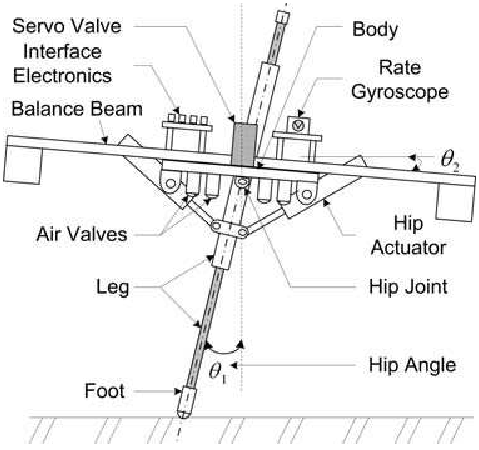
\includegraphics[width=0.4\textwidth]{fig/Rai_2D}}
  \hspace{2cm}
  \subfloat[ARL Monopod I \cite{ARLMono1}] {\label{fig:1_mono1_hip}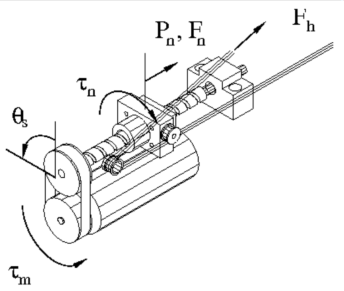
\includegraphics[width=0.450\textwidth]{fig/ARLMono1_hipmotor}}
  \caption[Actively stabilized hoppers]{Actively stabilized hoppers}
  \label{fig:1_activestable}
\end{figure}
\subsubsection{Actively Balanced Robots}
Raibert used a hydraulically actuated hip on top of an articulate leg mechanism for balancing the hopper. The hip actuator used in
the two-dimensional hopper shown in Fig. \ref{fig:1_rai_2D} was pneumatically controlled by varying the pressure gauged by pressure 
sensors on the actuators. The hip can also be moved by means of a winch type actuator as shown in Fig. \ref{fig:1_mono1_hip}. 

\subsubsection{Passive Balancing Robots}
Swinging the leg for active balancing requires energy and people started looking for ways to achieve passive stabilization of
hopper attitude. This kind of stabilization might not provide a complete solution to the problem of stability but certainly reduces
the power consumption of the robot.
After studying ARL Monopod I,  Beuhler incorporated a compliant spring in series with the hip actuator cables as shown in Fig. \ref{fig:1_ARLMono2_sch}. Swinging of the leg could be achieved using the hip-leg spring compliance. Thus a passively stable
running gait was possible for certain initial conditions \cite{Bue_PassRun, ARLMono2}.\\
\begin{figure}[h]
  \centering
  \subfloat[ARL Monopod II \cite{ARLMono2}]{\label{fig:1_ARLMono2_sch}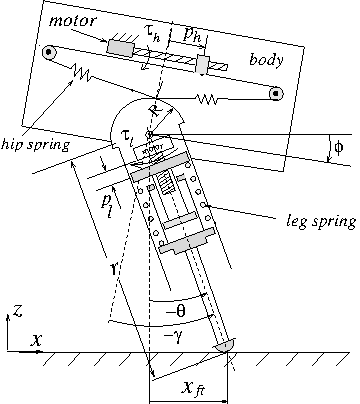
\includegraphics[width=0.4\textwidth]{fig/ARLMono2_sch}}
  \hspace{0.05\textwidth}
  \subfloat[SLOM hopper \cite{sayyad}]{\label{fig:1_SLOM}\includegraphics[width=0.4\textwidth]{fig/SLOM}}
  \caption[Passively dynamically stable hoppers]{Passively dynamically stable hoppers}
\end{figure}

Most of the hoppers reviewed in \cite{review} have their C.G. along the line of action of the impact and spring forces. This provides
a stable system for single place hopping and is referred to as \emph{Springy Leg Inverted Pendulum} (SLIP). It is noted that SLIP
does not account for the pitch stabilization problem which is of practical concern.\\

As shown in Fig. \ref{fig:1_SLOM}, Shanmuganathan et. al. considered asymmetric configurations in which the CG location was offset 
from the geometric center. This is referred to as a \emph{Springy-Legged Offset-Mass} (SLOM) hopper \cite{shanmug}. The robot 
postures at various phases during a hopping cycle are depicted in Fig. \ref{fig:4_rewac}. The impulsive torque acting during the 
stance gives a pitch up velocity in the flight phase. This compensates the net pitch down during the stance phase due to the 
horizontal velocity. Sayyad and Seth have analyzed this configuration using a 3D Poincar\'e map to obtain a periodic motion 
stabilized by observer based state feedback strategy \cite{sayyad}. Fig. \ref{fig:1_wei} shows a miniature 5 cmm tall SLOM hopper developed by
Wei et. al. \cite{5cmhopper}

\vspace{0.4in}
\begin{figure}[h]
\centering
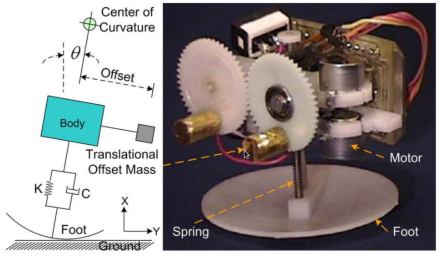
\includegraphics[scale=1]{fig/wei.pdf}
\caption[5 cm tall hopper by Wei]{5 cm tall hopper by Wei et. al. \cite{5cmhopper}}
\label{fig:1_wei}
\end{figure}

















